\section{Results}

\subsection{Implementation and verification}
Forward and backward passes are compiled with Numba; a PyTorch \texttt{autograd.Function} calls them, and a second, pure PyTorch version processes whole anti-diagonals at once ($n+m$ sequential steps instead of $nm$), which is the scheme GPU implementations use. We check the value and $E$ against \emph{brute-force enumeration of every alignment} (all Delannoy paths, $n,m\le5$, $\gamma\in[10^{-2},10]$, error $<10^{-10}$), the gradient against finite differences, the bound $\mathrm{dtw}-\gamma\log|\mathcal A|\le\sdtw\le\mathrm{dtw}$, the agreement with \texttt{tslearn}, and the custom backward against autograd. All variants scale as $O(nm)$ (fitted log-log slopes $2.02$--$2.04$), but constants differ by orders of magnitude: for $n=m=64$ forward+backward takes $0.3$\,ms with Numba, $20$\,ms with the same code in pure Python and $0.75$\,s with a cell-by-cell PyTorch forward differentiated by autograd, which confirms the paper's remark that a custom backward is essential. Fig.~\ref{fig:E} shows how $E$ moves from the hard DTW path ($\gamma\to0$) to a diffuse band, and for large $\gamma$ to a data-independent diagonal band.

\begin{figure}[t]
\centering
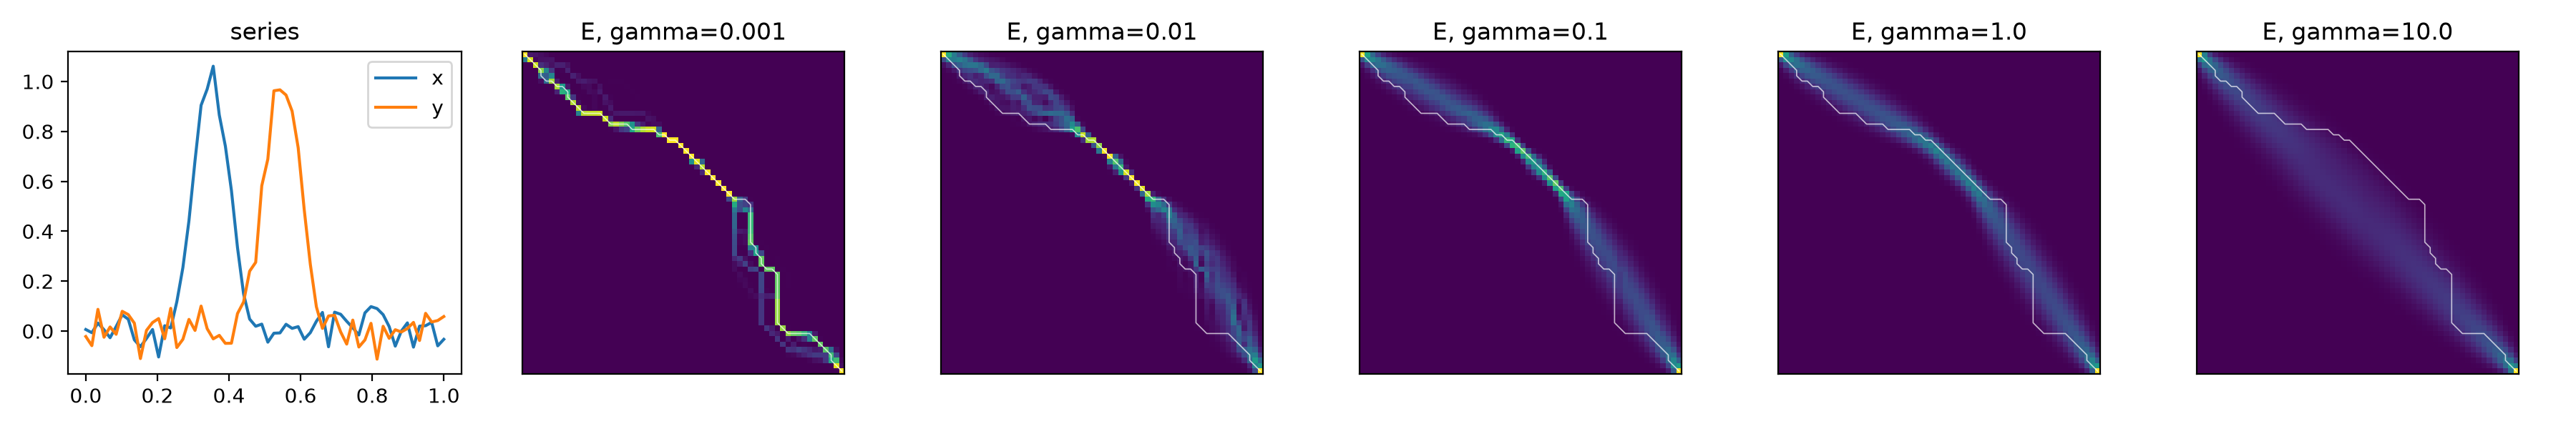
\includegraphics[width=\linewidth]{E_vs_gamma.png}
\caption{Expected alignment $E=\mathbb E_\gamma[A]$ between two shifted bumps for increasing $\gamma$; white: optimal DTW path. For $\gamma=10$ the alignment ignores the data and concentrates around the diagonal.}
\label{fig:E}
\end{figure}

\subsection{Barycenters and $k$-means (Tables 1--2 of the paper)}
Protocol as in the paper: for each dataset, 10 random draws of 10 series of one class; barycenters from the same initialisation (random $\mathcal N(0,1)$ or Euclidean mean) with at most 100 iterations; soft-DTW with L-BFGS, DBA~\cite{petitjean2011global} (\texttt{tslearn}) and a batch subgradient method with backtracking line search~\cite{schultz2018nonsmooth}. All methods are scored with the \emph{hard} DTW objective (Eq.~4 with $\gamma=0$), which is the objective DBA itself minimises. $k$-means uses $k$ = number of classes, at most 30 Lloyd and 100 barycenter iterations, training sets capped at 100 series, 3 random initialisations (random series) and a Euclidean $k$-means initialisation.

\begin{table}[t]
\centering\small
\caption{Percentage of datasets on which soft-DTW reaches a lower hard-DTW loss than DBA / the subgradient method. Ours (12 datasets for barycenters, 10 for $k$-means) vs.\ the paper (79 datasets) in parentheses.}
\label{tab:repro}
\setlength{\tabcolsep}{4pt}
\begin{tabular}{llcccc}
\toprule
& & $\gamma=1$ & $\gamma=0.1$ & $\gamma=0.01$ & $\gamma=0.001$ \\
\midrule
\multirow{4}{*}{Barycenters}
& vs DBA, random init & 58 (41) & 92 (94) & 100 (100) & 100 (97) \\
& vs DBA, Euclidean init & 8 (4) & 25 (47) & 75 (80) & 100 (90) \\
& vs subgrad., random init & 75 (96) & 100 (97) & 100 (97) & 100 (97) \\
& vs subgrad., Euclidean init & 17 (35) & 75 (72) & 92 (92) & 100 (97) \\
\midrule
\multirow{4}{*}{$k$-means}
& vs DBA, random init & 10 (16) & 50 (25) & 70 (60) & 90 (77) \\
& vs DBA, Euclidean init & 10 (29) & 10 (24) & 60 (55) & 90 (69) \\
& vs subgrad., random init & 20 (42) & 60 (58) & 100 (76) & 90 (96) \\
& vs subgrad., Euclidean init & 10 (46) & 10 (50) & 90 (66) & 100 (84) \\
\bottomrule
\end{tabular}
\end{table}

Table~\ref{tab:repro} reproduces the paper's trends closely: small $\gamma$ beats DBA almost always, $\gamma=1$ rarely does, and the gap is larger from a random start. The paper only reports win rates; magnitudes and costs nuance the picture. \emph{Barycenters:} from a random start the median soft-DTW/DBA loss ratio is $0.86$ ($\gamma=0.01$), down to $0.26$ on Plane ($\gamma=0.1$), where DBA is trapped in a poor local minimum; from the Euclidean mean, which is already a good start, the gain is only $3$--$4\%$ (median ratio $0.97$). \emph{$k$-means:} gains shrink further (median ratio $0.97$ for $\gamma\le0.01$). \emph{Cost:} with $\gamma=0.001$ a soft-DTW barycenter takes $14\times$ (and a $k$-means run $16\times$) the time of DBA, because the objective becomes nearly non-smooth and L-BFGS needs many more steps. Conversely, $\gamma=1$ gives visually smooth barycenters but losses up to $3\times$ that of DBA: smoothness and fidelity to DTW pull in opposite directions, and the hard-DTW metric only rewards the latter. Finally, the subgradient baseline is very sensitive to its step size (from a random start it stalls $30\times$ above DBA on Coffee and Trace), which inflates the win rates against it.

\subsection{Nearest-centroid classification (Fig.~7 of the paper)}
Following the paper, data are pooled and split 50/25/25 (3 random stratified splits) and $\gamma$ is selected on validation among 15 log-spaced values in $[10^{-3},10]$. Soft-DTW centroids are at least as accurate as DBA centroids on 83\% of the datasets (paper: 75\%), with mean accuracy $0.86$ vs $0.81$. Two baselines the paper does not report put this in context: Euclidean centroids reach $0.77$, but \textbf{1-NN DTW reaches $0.93$} and is better than soft-DTW centroids on 9 of 12 datasets. Nearest centroids trade accuracy for a much smaller model and faster prediction. Moreover, the selected $\gamma$ is unstable: on CBF it ranges from $0.002$ to $0.19$ across splits, and on ECGFiveDays the largest value $\gamma=10$ is always selected, i.e.\ there is no reliable default for $\gamma$.

\subsection{Multistep-ahead forecasting (Table 3 of the paper)}
\todo{results of exp\_forecast: average ranks, Euclidean vs DTW test metrics, qualitative figure (ShapesAll)}

\subsection{A family of soft alignment distances}
\todo{results of exp\_family: 1-NN accuracy of soft-DTW / soft-ADTW / soft-WDTW / soft-ERP, raw vs divergence, vs Euclidean and 1D Wasserstein controls; selected gamma and omega}
